\counterwithin{figure}{Appendix}
\counterwithin{table}{Appendix}
\counterwithin{equation}{Appendix}
% \renewcommand{\thefigure}{\theAppendix.\arabic{figure}}
% \renewcommand{\thetable}{\theAppendix.\arabic{table}}
% \renewcommand{\theequation}{\theAppendix.\arabic{equation}}
\begingroup
\centering

\Appendix\label{appendix:lights}
% \fancyfoot[R]{}
План помещения и размещения светильников с люминесцентными лампами
\begin{figure}[h]
    \centering
    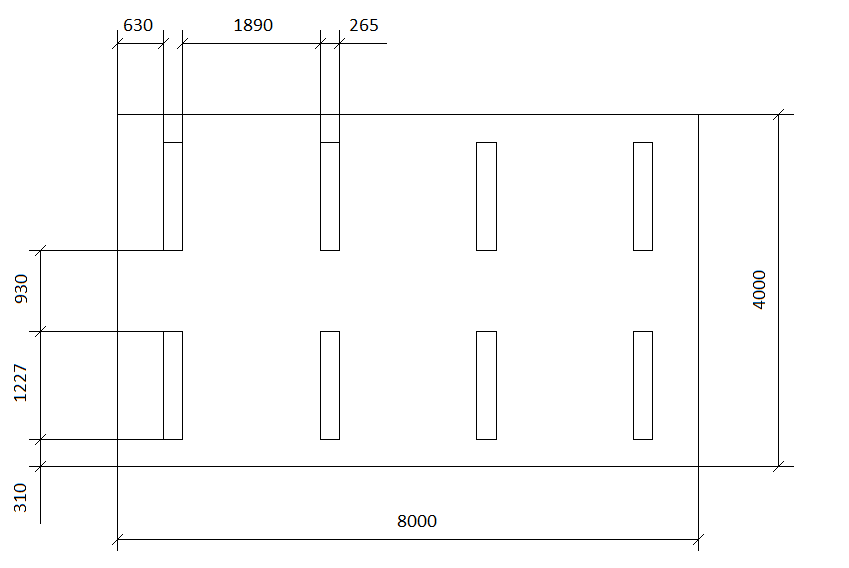
\includegraphics[width=\textwidth]{Lamps.png}
\end{figure}

\begin{landscape}
\Appendix\label{appendix:evacuation}
План эвакуации в случае пожара
\begin{figure}[h]
    \centering
    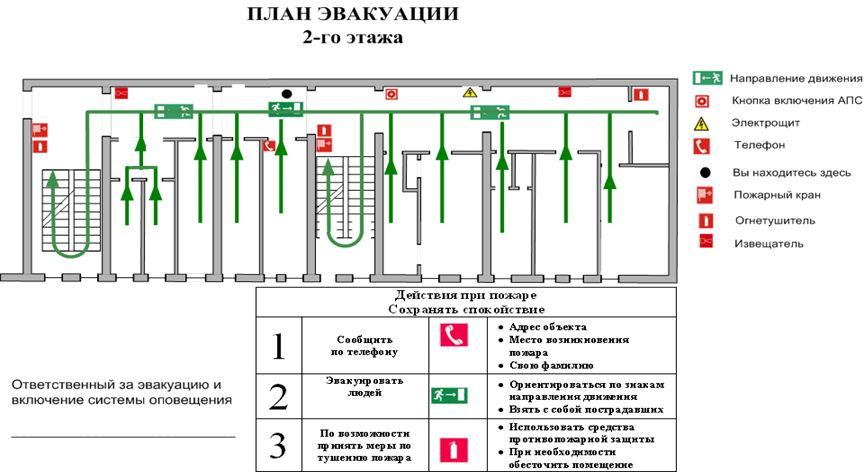
\includegraphics{Evacuation.png}
\end{figure}
\end{landscape}

\endgroup

\Appendix\label{appendix:eng1}
\begingroup
\singlespacing
\centering
\AtBeginEnvironment{tabularx}{\setstretch{1}}
\renewcommand\tabularxcolumn[1]{p{#1}}

\vspace{\fill}
\vspace{\fill}

\textbf{Portfolio risk assessment using copula models}
% Раздел~\ref{section:literature}

% Обзор литературы

\small
\vspace{\fill}

\begin{tabularx}{\textwidth}
{|>{\hsize=0.64\hsize}Y|>{\hsize=2.08\hsize}Y|>{\hsize=0.64\hsize}Y|>{\hsize=0.64\hsize}Y|}
    \multicolumn{4}{l}{Студент} \\
    \hline
    \scriptsize \textbf{Группа}
        & \scriptsize \textbf{ФИО}
        & \scriptsize \textbf{Подпись}
        & \scriptsize \textbf{Дата} \\
    \hline 
    0ВМ61\bigstrut & Смагулов Даулет Серикбаевич & & \\ 
    \hline
\end{tabularx}

\vspace{2ex}

\begin{tabularx}{\textwidth}
{|>{\hsize=1.7\hsize}Y|>{\hsize=1.0\hsize}Y|>{\hsize=0.9\hsize}Y|>{\hsize=0.7\hsize}Y|>{\hsize=0.7\hsize}Y|}
    \multicolumn{5}{l}{Консультант отделения экспериментальной физики ИЯТШ:} \\
    \hline
    \scriptsize \textbf{Должность} 
        & \scriptsize \textbf{ФИО} 
        & \scriptsize \textbf{Учёная степень, звание} 
        & \scriptsize \textbf{Подпись} 
        & \scriptsize \textbf{Дата} \\
    \hline
    доцент отделения экспериментальной физики & Семёнов М. Е.\bigstrut & к. ф.-м. н., доцент & & \\ 
    \hline
\end{tabularx}

\vspace{2ex}

\begin{tabularx}{\textwidth}
{|>{\hsize=1.7\hsize}Y|>{\hsize=\hsize}Y|>{\hsize=0.9\hsize}Y|>{\hsize=0.7\hsize}Y|>{\hsize=0.7\hsize}Y|}
    \multicolumn{5}{l}{Консультант-лингвист отделения иностранных языков ШБИП:} \\
    \hline
    \scriptsize \textbf{Должность} 
        & \scriptsize \textbf{ФИО} 
        & \scriptsize \textbf{Учёная степень, звание} 
        & \scriptsize \textbf{Подпись} 
        & \scriptsize \textbf{Дата} \\
    \hline
    старший преподаватель отделения иностранных языков & Смирнова У. А.\bigstrut & & & \\ 
    \hline
\end{tabularx}

\vspace{\fill}

\endgroup

\begingroup
\captionsetup*[figure]{name={Figure}}
\captionsetup*[table]{name={Table}}
\renewcommand{\algorithmicrequire}{\textbf{Input:}}
\renewcommand{\algorithmicensure}{\textbf{Output:}}
\floatname{algorithm}{Algorithm}

\begin{english}
\begingroup
\singlespacing
\centering
\small
\AtBeginEnvironment{tabularx}{\setstretch{1}}
\AtBeginEnvironment{tabular}{\setstretch{1}}
\AtBeginEnvironment{longtable}{\setstretch{1}}
\renewcommand\tabularxcolumn[1]{p{#1}}

\vspace{\fill}
\vspace{\fill}

Раздел~\ref{section:literature}

Обзор литературы

\vspace{\fill}

\begin{tabularx}{\textwidth}
{|>{\hsize=0.64\hsize}Y|>{\hsize=2.08\hsize}Y|>{\hsize=0.64\hsize}Y|>{\hsize=0.64\hsize}Y|}
    \multicolumn{4}{l}{Студент} \\
    \hline
    \scriptsize \textbf{Группа}
        & \scriptsize \textbf{ФИО}
        & \scriptsize \textbf{Подпись}
        & \scriptsize \textbf{Дата} \\
    \hline 
    0ВМ61\bigstrut & Смагулов Даулет Серикбаевич & & \\ 
    \hline
\end{tabularx}

\vspace{2ex}

\begin{tabularx}{\textwidth}
{|>{\hsize=1.8\hsize}Y|>{\hsize=1.1\hsize}Y|>{\hsize=0.7\hsize}Y|>{\hsize=0.7\hsize}Y|>{\hsize=0.7\hsize}Y|}
    \multicolumn{5}{l}{Консультант школы отделения (НОЦ):} \\
    \hline
    \scriptsize \textbf{Должность} 
        & \scriptsize \textbf{ФИО} 
        & \scriptsize \textbf{Учёная степень, звание} 
        & \scriptsize \textbf{Подпись} 
        & \scriptsize \textbf{Дата} \\
    \hline
    & {}\bigstrut & & & \\ 
    \hline
\end{tabularx}

\vspace{2ex}

\begin{tabularx}{\textwidth}
{|>{\hsize=1.8\hsize}Y|>{\hsize=1.1\hsize}Y|>{\hsize=0.7\hsize}Y|>{\hsize=0.7\hsize}Y|>{\hsize=0.7\hsize}Y|}
    \multicolumn{5}{l}{Консультант-лингвист отделения (НОЦ):} \\
    \hline
    \scriptsize \textbf{Должность} 
        & \scriptsize \textbf{ФИО} 
        & \scriptsize \textbf{Учёная степень, звание} 
        & \scriptsize \textbf{Подпись} 
        & \scriptsize \textbf{Дата} \\
    \hline
    старший преподаватель отделения иностранных языков & Смирнова У. А.\bigstrut & старший преподаватель & & \\ 
    \hline
\end{tabularx}

\vspace{\fill}

\endgroup


\anonsection{Literature review}

Common measures of risk used in risk management are "value-at-risk" (\textit{VaR}) and "conditional-value-at-risk" (\textit{CVaR}) which can be determined for different levels of significance. 
It is noted in the paper \cite{Kritski2007} that in the presence of a correlation of Profit \& Loss series of assets, one-dimensional risks' measures \textit{VaR} and \textit{CVaR} assess the portfolio risk incorrectly, see, e.g.,~\cite{Rachev2005}. 
Therefore, to assess the portfolio risk, it is necessary to use $d$-dimensional measures determined through the multivariate dependence.

There are many different approaches that actively used in applications to represent multivariate dependence, for instance, principal component analysis, Bayesian networks, fuzzy techniques, factor analysis, and joint distribution function, \cite{Huynh2014, Kole2007}. 
The dependence among the random variables $x_1, x_2, \ldots, x_d$, is completely described by the joint distribution function $F_X(x_1, x_2, \ldots, x_d)$. 
The idea of separating $F_X(x_1, x_2, \ldots, x_d)$ in two parts -- the one which describes the dependence structure, and the other one which describes the marginal behavior, leads to the concept of copula.

In 1959, A.~Sklar~\cite{Sklar1959} first proved the theorem that a collection of marginal distributions can be coupled together via a \textit{copula} to form a multivariate distribution.
The copula contains all the information about the dependence structure of the involved variables.
In the paper~\cite{Penikas2010}, the author introduced copula-models' concepts and its application to the different financial issues including the task of risk measurement.

Many ways to describe financial data using Gaussian (normal) distribution exist today. 
It is well known from \cite{Xu2008} that a full Gaussian copula, i.\,e., a Gaussian copula constructed by Gaussian (normal) marginals, is another way to describe Markowitz's mean-variance portfolio theory. 
On the other hand, a lot of empirical studies have shown that Gaussian distribution has a lot of problem in dependence description of financial data, see, e.g., \cite{Rachev2005, Limp2011, Wilmott2007, Pourkhanali2016}. 
Moreover, in the standard \cite{EBA2015} is proposed that Gaussian copulas are not to be used for operational risk modelling. 
For instance, a Student's~$t$ copula with few integer degrees of freedom (three or four) in most cases appears more appropriate.
Closed-form expressions to calculate the sensitivity of the risk measure, \textit{CVaR}, were proposed in the paper by \cite{Stoyanov2013}.

Studies of price risks in framework of portfolio management \cite{Ane2003, Kole2007, Lourme2016, Xu2008} in many respects are similar to each other and differ only in the used data and insignificant variations in the copula models estimation. 
Among the studies, we single out the paper by \cite{Ane2003} that was one of the first one where authors selected the dependence structure of international stock index returns through the Clayton copula. 
\cite{Lourme2016} address the issue of testing the full Gaussian and Student's~$t$ copulas in a risk management framework. 
They proposed the $d$-dimensional compact Gaussian and Student's~$t$ confidence area inside of which a random vector with uniform margins on $(0, 1)$ falls with probability~$\alpha$. 
The results evidence that the Student's~$t$ copula \textit{VaR} model is an attractive alternative to the Gaussian one.
A portfolio of stocks, bonds and real estate was considered by \cite{Kole2007} to determine the importance of selecting the right copula for risk management. 
The Gaussian, the Student’s~$t$ and the Gumbel copulas to model the dependence of the daily returns on indexes that approximate these three asset classes were tested. 
Then with Value-at-Risk computations was established that the Gaussian copula is too optimistic on the diversification benefits of the assets, while the Gumbel copula is too pessimistic.  

Estimation of the unknown parameters is an important problem. 
At present, many algorithms for constructing copulas have been designed.
For copula model estimation, there exist three methods: the full parametric method \cite{Patton2006}, the semi-parametric method \cite{Lourme2016, Chen2006}, and the non-parametric method \cite{Fermanian2003, Kim2007}.
The full parametric method is implemented via two-stage maximum likelihood estimation (MLE) proposed by \cite{Joe1997, Joe2014}. %(1997, 2005, 2014).
The copula is fitted using the two-stage parametric MLE approach, also referred to as the Inference Functions for Margins (IFM) method.
This method fits a copula in two steps: (1) estimate the parameters of the marginals, and (2) fix the marginal parameters to the values estimated in first step, and subsequently estimate the copula parameters.

For the the bivariate case, the main families of copulas are: ellipse (Gaussian, Student's~$t$), archimedean (Clayton, Frank, Joe), and extreme (Gumbel, Cauchy).
In the dissertation research \cite{Xu2008}, the two-stage  MLE method was applied, while the author uses all possible combinations of different marginal distributions (Gaussian, the Student's $t$, and skewed $t$ distribution) and different archimedean copulas in the estimation and testing process. 
The decision of choosing the marginal distribution is taken after the second step of MLE method.
For this purpose, a modification of the superior predictive ability of the Hansen test was proposed \cite{Hansen2005}; it allows one to identify a copula that has superior forecasting ability.

Multivariate copulas based on the one distribution (for instance, normal or Student's~$t$) or on one the generator function lack the flexibility of accurately modeling the dependence among larger numbers of variables \cite{Brechmann2013}. 
These lacks predetermined the direction of further research, as a result of which the regular vine copulas' (R-vine) concept was proposed by \cite{Joe1996} and developed in more detail by \cite{Brechmann2013, Cooke2015}.
R-vine copulas are a flexible graphical model for describing multivariate copulas built up using
a cascade of bivariate copulas (two-dimensional function). 
This copula is easier to be interpreted and visualized, and we have a lot of methods to work with it today \cite{Nikoloulopoulos2012, Cooke2015, Czado2010, Dissmann2013}. 
\cite{Nikoloulopoulos2012} applied the vine copulas with asymmetric tail dependence for financial return data.
A novel algorithms for evaluating a \textit{regular vine copula} parameters and simulating
from specified R-vines were proposed by \cite{Dissmann2013}. 
The selection of the R-vine tree structure based on a maximum spanning tree algorithm (MST), where edge weights are chosen appropriately to reflect large dependencies.
\cite{Pourkhanali2016} proposed the use of vine copula for measuring systemic risk, they developed a metric that captures crucial features of the dependence relationship: tail-dependence and correlation asymmetry.
\end{english}
\endgroup